%
%  This document contains chapter 2 of the thesis.
%
\documentclass[cs,msthesis]{usuthesis}

\documentclass[cs,msthesis]{usuthesis}

%{{{ Packages
\usepackage{amssymb}           % add ams symbols stuff
\usepackage{graphicx}          % add graphics
\usepackage{subcaption}
\usepackage{url}
\usepackage{flafter}           % Cause floats to appear after
                               % environment.
                               % MDH: This was originally commented out.
%\usepackage{siunitx}           % Provides standard formatting of SI units.
\usepackage{listings}          % Use when including computer code.

% Include TikZ and PGF packages for high-quality graphics, schematics
% and plots. This is optional; at the current time, when run with
% latex to create a .dvi file, the xdvi viewer will produce incorrect
% formatting for the TikZ figures.  If the .dvi file is converted to
% pdf using "dvipdf" the resulting pdf file is correct.  If this
% example is used with  pdflatex, the resulting TikZ figures in the
% output look fine.
\usepackage{tikz}       		% The base tikz+pgf package
\usetikzlibrary{arrows,shapes}	% Optional tikz extensions
\usepackage[american]{circuitikz}	% TikZ-based package for schematic drawings
\usepackage{pgfplots}			% Tikz-based package for making plots
\pgfplotsset{compat=1.6}        % This *might* be necessary for your
                                % version of pgfplots.

\usepackage{hyperref} % Creates hyperlinks within document
\hypersetup{colorlinks=true, linkcolor=blue,
    citecolor=blue,urlcolor=blue} % Use when compiling the digital copy
% \hypersetup{colorlinks=true, linkcolor=black,
% citecolor=black,urlcolor=black} % Use when compiling the printed copy

% The following allows for hyperlinked DOIs to be inserted in the
% manuscript by using \doi{}.
\usepackage{doi}

\usepackage{enumitem} % MDH: Used for more controls over `enumerate`
\usepackage{amsmath} % MDH: For math functions
\usepackage{amsfonts} % MDH: For math fonts

\usepackage{util} % MDH: Contains my custom commands
\usepackage{notations} % MDH: So I don't have to repeat myself so much
\usepackage{hhline}  % MDH: For double lines in tables
\usepackage{tkz-euclide}  % MDH: To make it easier to label points in Tikz
\usepackage{xfrac}  % MDH: Additional fraction commands
\usepackage{makecell}  % MDH: Better controls in tables
\renewcommand\theadalign{bc}
\renewcommand\theadfont{\bfseries}
\renewcommand\theadgape{\Gape[4pt]}
\renewcommand\cellgape{\Gape[4pt]}
\usepackage{pifont}

% To control where figures are output
\usepackage{epstopdf}
\pdfminorversion=7 % Because epstopdf outputs as version 1.7


% Set spacing around figures and tables to triple space
\setlength{\intextsep}{2em} % Vertical space above & below [h] floats
\setlength{\textfloatsep}{2em} % Vertical space below (above) [t] ([b]) floats

% The following is added if you are using the multiple-paper format to
% add references after each chapter:
\usepackage[sectionbib]{chapterbib}

\newcommand{\vicki}[1]{\textcolor{blue}{Vicki: #1}}

\usepackage{pdflscape}

% Author and Title Information
\author{Michael D. Hegerhorst}
\title{
    Proxy Voting Coordination Mechanisms:\\
    Determining How Agents should Coordinate in a Continuous Preference Space
}

% The Committee
\majorprof{Vicki Allan, Ph.D.}
\firstreader{John Edwards, Ph.D.}
\secondreader{Shuhan Yuan, Ph.D.}
%\thirdreader{Gottfried Liebniz, Ph.D.}
%\fourthreader{Isaac Newton, Ph.D.}

% Graduate Dean
% TODO: Add the name and title of the CS graduate dean
\graddean{FIX ME: CS GRADUATE DEAN}
\deantitle{FIX ME: CS GRADUATE DEAN}

% Degree Information
% TODO: Should this be "Master of Science in Computer Science?"
\degree{Master of Science}
\month{April}
\gradyear{2023}


\begin{document}
    %{{{ Frontmatter
\preliminaries   % set frontmatter style

\maketitle
\makecopyright        % optional

%
%

\begin{abstract}
% A space is needed before the text starts so that the first paragraph
% is indented properly. Max 350 words.

    % TODO: Rewrite
    In May 2020, the 116th United States Congress passed a resolution to permit the
    use of proxy voting during emergencies for members of the House of Representatives.
    Proxy voting is a system of voting where a voter can assign another voter, called
    a proxy, to vote on their behalf.
    As with other voting systems, the votes are then aggregated into a final result
    using a voting rule or mechanism.
    Ideally, the result of proxy voting would be the same, or as close to as
    possible, to the result if everyone were to vote.
    This resolution was almost immediately put into practice and remains active at
    the time of this study.
    While it was designed to reduce the transmission of disease such as COVID-19, if
    proxy voting can be shown to be beneficial the resolution could be expanded to
    create a more efficient government system.
    However, proxy voting in Congress has been regarded with some skepticism and the
    question remains as to if proxy voting has too great of an effect on the result
    of the vote.
    In this study, we give proxy voting its best chance and explore its effects on
    the results of the vote under a number of opinion distributions.
    We additionally explore how different voting rules affect the results of the vote.
    We employ an opinion space model and determine the result of a vote as a point in
    the model space, instead of the vote simply passing or failing, in order to
    increase the granularity of the results and determine how much error is
    introduced due to proxy voting.
    Finally, we attempt to determine under which circumstances proxy voting should be
    used, if any, and identify strengths and weaknesses of using proxy voting in the
    modern House of Representatives.
    % TODO: Put in a bit of what we discover


\end{abstract}


% Local Variables:
% TeX-master: "newhead"
% End:

%
%  Time-stamp: "[publicabstract.tex] last modified by Scott Budge (scott) on 2011-08-09 (Tuesday, 9 August 2011) at 09:17:43 on goga"
%
%  Info: $Id$   USU
%  Revision: $Rev$
% $LastChangedDate$
% $LastChangedBy$
%

\begin{publicabstract}
% A space is needed before the text starts so that the first paragraph
% is indented properly.

Proxy voting is a type of voting where individuals are able to pass their votes to
someone else so they may vote for them.
This type of voting system allows for those without the time or knowledge necessary
to become informed on a topic to pass their votes to an individual they trust who
knows more about the topic, dubbed an expert.
This study investigates the ability of proxy vote systems to be used as a way to make
taking measurements more accurate by allowing less expensive measurements to pass their
vote on to more expensive `expert' measurement techniques.


\end{publicabstract}


% Local Variables:
% TeX-master: "newhead"
% End:
 % TODO: Update
%
% Dedication
%

\begin{dedication}
% \begin{center}
    To Danielle, my constant companion and eternal partner.
    
    You are my light and my star, my guiding hope.
    I love you.
\newline
\newline

    And to Miriam, who joined us in our adventure.
    
    May you lift others up and help them to be as brilliant as you.
% \end{center}
% 
% If you intend to have a dedication longer than one line, do not put
% it in a centering environment.  It will look better.
\end{dedication}
  % optional
%%
% This is an example of an acknowledgements page.  This is optional,
% and can contain anything you want to say.
%
%
%  Time-stamp: "[acknowl.tex] last modified by Scott Budge (scott) on 2011-08-08 (Monday, 8 August 2011) at 15:45:15 on goga"
%
%  Info: $Id$   USU
%  Revision: $Rev$
% $LastChangedDate$
% $LastChangedBy$
%

\begin{acknowledgments}
FIX ME
\\
\begin{flushright} 
Michael D. Hegerhorst
\end{flushright}
\end{acknowledgments}

     % optional TODO: Do I want acknowledgements?

\tableofcontents
\listoftables
\listoffigures

% %
% Contains notations used in this paper.
% Mostly used because I hate having to search throughout a paper to figure
% out what a symbol means in a math equation.
%
%! suppress = EscapeAmpersand
\newcommand{\notationheader}[1]{\multicolumn{2}{l}{\textbf{#1}}\\}
\newcommand{\notationdesc}[2]{#1 & #2\\}

\begin{notation}
\setlength{\tabcolsep}{3mm}{
    % TODO: Alphabetize these by symbol
    \begin{tabular}{ll}
        \notationheader{Equations}
        \notationdesc{\agent}{An individual agent}
        \notationdesc{\agentcost}{The cost of using an individual agent}
        \notationdesc{\agents}{The set of all agents}
        \notationdesc{\cost}{Cost}
        \notationdesc{\loss}{Loss}
        \notationdesc{\real}{The set of all real numbers}
        \notationdesc{\system}{A system}
        \notationdesc{\systemspace}{The space within a system operates}
        \notationdesc{\truth}{Truth}
        \notationdesc{\agenttruth}{The truth as estimated by an agent}
        \notationdesc{\systemagents}{The agents of a system}
        \notationdesc{\systemcost}{The cost of a system}
        \notationdesc{\systemloss}{The loss of a system}
        \notationdesc{\systemtruth}{The truth as estimated by a system}
    \end{tabular}
}

% The table as defined above will fill one page. If you need more room to list
% notation you will need to create a second table, and place it below this 
% comment. This new table will appear one a new page.

\end{notation}

  % optional TODO: Update
% \include{content/frontmatter/acronyms}  % optional TODO: Update
%}}}

    %{{{ The main body of the thesis
    \body  % set main body style
    % Chapters
    \chapter{RESULTS}\label{ch:results}
    %%%%%%%% This line gets rid of page number on first page of text
    \thispagestyle{empty}
    %%%%%%%%%%%%%
    From determining the best breakfast cereal~\cite{Curtis2021} to electing the next
    president, voting is an extremely important aspect of modern society.
    Nevertheless, disease, injury, and other impediments can create difficulties for
    individuals participating in such democratic processes, preventing them from
    expressing their voice and participating in deliberation, as well as decreasing
    the overall quality of the result.
    Proxy voting is a method by which participants are able to have others vote on their
    behalf.
    We examine the ability of proxy voting to decrease the impact of such frustrations.
    We additionally determine strategies by which proxies and their constituents can
    cooperate in order to reduce the change their absence would otherwise cause.
    These strategies include allowing proxies and constituents to aggregate their
    preference into one result, as well as determining how best to aggregate all votes in
    a unified-vote/single-winner/single-dimension continuous space model.

    \section{Background}\label{sec:background}

\subsection{What is proxy voting?}\label{subsec:what-is-proxy-voting?}
\textit{Proxy voting} is a group of methods by which individuals who are unable or
uninterested in voting in person can still have their voices heard through the use of
a \textit{proxy}, who is an individual authorized to act for another.
Agents are able to delegate another individual to be their proxy.
We call the delegating agent a \textit{delegator} or an \textit{inactive voter}, and
the group of agents that delegate to a proxy its \textit{constituents}.
Proxies are also known as \textit{delegates} or \textit{active voters}.

When voting, each individual starts with a certain number of votes that it can
allocate to any given option.
Typically, this number is one.
The number of votes a voter has are called its \textit{weight} or \textit{voting power}.
For example, an individual with a weight of $n$ who votes for $x$ has the same impact
as if $n$ distinct voters with a weight of 1 picked $x$.
When delegating a proxy, the delegator's weight is transferred to the proxy,
increasing their total weight by the amount of power transferred.
The more weight a voter has, the more they can swing the vote in their favor.

Upon selecting a proxy, a delegator is no longer able to vote directly.
Instead, their delegate votes on their behalf.
In contrast, \textit{direct voting} requires each agent to vote on their own, meaning
each agent must incur the costs of voting or not have their voice heard.
These costs may be tangible, such as needing to pay for gas, or intangible, such as
the time or effort required to vote in-person.
Such costs are common in voting, and are further discussed by~\cite{Gershtein2019}.
Error is introduced into the result of direct voting when an agent is unable or
unwilling to pay these costs, since information is lost when agents do not share
their preference via a vote.
In votes with discrete options, this error could be anything from a different result
(in the worst case) or a slightly different count of the votes (for example, 10
votes in favor instead of 11).
In these cases, such as in times of injury or illness, proxy voting provides an
excellent avenue through which the agent can still have its voice heard and reduce
the error in the system.

Proxy voting is beneficial for the delegates as well.
By working on behalf of their constituents, a proxy has a larger voice in discussions
and deliberations since they are representing more agents.
This allows them to have a larger influence and achieve a greater impact as topics
are debated.

Proxy voting systems are not, however, without flaws.
When agents do not participate in person, they are not able to participate in
deliberation.
Such discussions are vital to the voting process, since as agents confer, they gain
access to new information which may change their preference.
Inactive agents do not benefit from this deliberation; only active agents do.
As such, proxies have to participate in deliberation and change their preference on
behalf of their constituents.
It is possible the proxy will change its preference in such a way that some of its
constituents would not.
If the proxy is only allowed to cast one vote on behalf of all its constituents, those
constituents will have their vote applied in a way they find less preferable than
simply paying the costs.
In this `unified-vote' model, an agent must choose a proxy they are confident would
change their preference in the same way they would `if only [they] had the time and
knowledge to participate directly'~\cite{Miller1969}, or risk having their vote
misallocated.
When a vote is misallocated, error is again introduced into the system, and may
arguably be worse than if the inactive agent hadn't voted at all since it may change
the result of the vote from what it would with all agents participating.

As an alternative to only casting one vote on behalf of all constituents, the proxy
could be allowed to vote once per constituent, and can even be required to vote
precisely as each constituent requests.
This is the system the 116th United States Congress introduced in May 2020 in an
attempt to reduce the risk of COVID-19 in the House of
Representatives~\cite{CERP2020, Congress.gov2020}: the proxies effectively `relay' their
delegators' votes individually and for each inactive voter.
As such, information about the inactive voters' preferences is not lost.
The process is effective in that every voter will have their vote allocated exactly
as they want, but comes with the obvious downside that each proxy has to keep track
of how each individual constituent wants their vote relayed.
This naturally increases the complexity and work required by the proxy.
Additionally, the inactive voters still need to be active in the deliberation process
in order to properly participate in the process.
This makes `relay-voting' only effective for occasions when agents have been able to
participate in the full process except for the voting itself and know exactly how
they want their vote allocated.

In this study, we will tackle some of the problems associated with unified-vote proxy
voting.
By determining methods to minimize the error produced by the model, the system will
yield the benefits of unified-vote deliberation while still producing a near-perfect
result.

    \section{Preliminary Setup}\label{sec:preliminary-setup}

\subsection{The Model}\label{subsec:the-model}
An important part of any study is the model it uses to represent the system being
studied.
We employ a model described by \etal{Cohensius} in their 2017
article~\cite{Cohensius2017}.
This model places voters' preferences in a single-dimension continuous
metric~space~\systemspace, such as in~\autoref{fig:system-metric-space}.
In this model, two points that are close together in the metric space represent
similar preferences, while two points that are far apart represent very different
preferences.
As a point moves further away from the agent's preference, the agent likes it less.
This model works best when an upper and lower bound is provided, such as only
allowing agents to vote in the interval $[-1, 1]$, to prevent agents from voting
extremely far in either direction and so potentially biasing the vote.
Not all methods of voting are susceptible to such attacks, but it must be a
consideration for those that are.

The difference between multiple equidistant points in the model may not be equivalent
to the agents.
For example, an agent who must spend \$30 may prefer spending more money rather than
less.
As such, even though \$29 and \$31 are equidistant to \$30, an agent may vastly
prefer \$31 over \$29.
However, for our model, we will assume agents only care about the distance from their
preference, rather than if it is greater or less than some amount.

\begin{figure}[htbp]
    \centering
    % Built using:
% https://tex.stackexchange.com/a/148253/277236
% https://tex.stackexchange.com/a/380491/277236
\begin{tikzpicture}[scale=7.0]
    \draw(-1,0) -- (1,0) ; % Axis
    \foreach \x in {-1, 0, 1} % Numbers and lower lines
    \draw[shift={(\x,0)},color=black] (0pt,2pt) -- (0pt,0pt);
    \foreach \x in {-1, 0, 1} % Numbers and lower lines
    \draw[shift={(\x,0)},color=black] (0pt,0pt) -- (0pt,-2pt) node[below]{$\x$};

    % Labeled points
    \tkzDefPoint((-4/7), 0){agentA}
    \tkzDefPoint((3/4) , 0){agentB}
    \tkzDefPoint((1/12), 0){agentC}
    \tkzLabelPoint[above](agentA){$\truthof{a}$}
    \tkzLabelPoint[above](agentB){$\truthof{b}$}
    \tkzLabelPoint[above](agentC){$\truthof{c}$}

    \foreach \n in {agentA, agentB, agentC}
    \node at (\n)[circle,fill,inner sep=1.75pt]{};
\end{tikzpicture}
    \caption{
        Example of a 1D continuous preference metric space, where \truthof{x} represents
        the preference of agent $x$.
        The x-axis represents some preference space.
        An agent can have a preference anywhere within this space.
        One way to interpret the model is to have the leftmost point be the most
        against some idea and the rightmost point is the most in favor of the same idea.
        Importantly, points towards the center of the space are the most ambivalent,
        neutral, or central on the idea.
        Alternatively, points towards the center may also prefer some type of
        compromise or alternative solution instead.
    }
    \label{fig:system-metric-space}
\end{figure}

Such a model is extremely flexible and can be interpreted in different ways.
When applied to binary for-or-against voting problems, options can be placed at either
extreme of the interval.
As an example, shareholders at some company are voting on new data collection policies.
Using the interval $[-1, 1]$, we can place `no collection at all' at -1, and `heavy
collection' at 1.
Agents vote according to their preference: -1 for no collection, 1 for heavy collection.
So far, everything works the same as a normal vote.
However, due to the continuous nature of the voting space, the agents can vote
anywhere in the given interval.
Therefore, agents who do not care one way or the other can vote at 0 instead of being
forced to choose an option.
Additionally, those that are only slightly in favor (meaning they would prefer
collection but do not really care that much) can choose some value between 0 and 1.
Once the votes are aggregated, the result can be rounded to whichever option is
closest.
The continuous space allows agents to better express themselves according to what
their actual preference is, instead of being forcibly binned into one value or the
other.

Alternatively, if the majority of the votes are about the center, it may be a sign
neither option is satisfactory.
Using the data collection example, we can reinterpret 0 to mean the agents do not
mind collecting users' data, but also do not personally care either way.
These agents would vote around 0 to avoid imposing.
By making the agents aware of how 0 will be interpreted, they can express their
dissatisfaction by voting at or around 0.
Normally, voting goes through a bargaining and an enforcement
phase~\cite{Fearon1998}, but if a sufficient number of agents vote close to 0, the
group can reopen discussion about the topic and re-bargain before conducting a new vote.
This enhances the cooperation aspect of voting, and creates a fundamental change:
voting is no longer the end of the negotiation, but rather part of it.

Finally, the continuous space model allows for another, very powerful interpretation:
interpreting the votes and result as continuous values.
For example, imagine Congress is voting on how much to allocate to the defense budget.
In this scenario, Congress can decide to allocate anywhere between \$0 and \$1,000.\footnote{
    Naturally, these values are not realistic and are meant to be representative.
}
A voter can place their vote anywhere between those values, and the result of the
vote can be how much Congress allocates.
Say there are three voters, each with their own preferences, and all voters are
active (no voter delegates their vote).
Agent $a$ prefers \$750, $b$ prefers \$600, and $c$ prefers \$250.
One way we could aggregate these preferences is by finding their mean.
By averaging these preferences, the system would output
$\frac{\$(750 + 600 + 250)}{3 \text{ voters}} = \frac{\$1600}{3 \text{ voters}} =
\$533.33$,
which would be the amount allocated to the defense budget.
Being able to vote on continuous problems and yield a continuous output, as well as
working with binary issues, makes the model extremely flexible and allows it to
tackle any number of problems.

We are also able to easily calculate error using a continuous space.
The error can simply be the distance from the result of the system when all agents
are active, and the result under proxy voting.

The flexibility of the continuous model in both the discrete and continuous realms, its
ability to use different voting rules, easy interpretability, and easy error
calculation are the reasons it is employed in this study.
We will focus primarily on the continuous instead of the discrete output of the
model, since observing the continuous output allows for more granularity in the
differences between proxy and non-proxy voting, as well as in the differences between
voting rules.

\subsection{Voting Mechanisms}\label{subsec:voting-mechanisms}
This study also makes use of \textit{voting mechanisms} or \textit{voting rules},
which are functions that map a set of preferences in~\systemspace\ to an outcome that
also exists in~\systemspace.
For these, we take inspiration from \etal{Bulteau}'s~\cite{Bulteau2021} work in
aggregating one-dimensional single-winner elections by using their $L_p$ aggregation
methods, as well as mixing in plurality.
$L_p$ aggregation methods work by minimizing the sum of distances to the power of $p$
($d^{\,p}$, where $d$ is a distance) between a possible solution and the voters'
preferences.
Naturally, since~\cite{Bulteau2021} did not use weighted proxies, these methods need
to be adjusted to allow for weight.
Below, \agentweight\ represents the weight of an agent \agent, and \systemproxies\ is
the set of active voters ordered by preference.
Additionally, \agenttruth\ is the preference of an agent, and \system\ is the set of
all agents.
With these notations, the mechanisms we use are
\begin{enumerate}
    \item {
        \textit{Median ($L_1$)}, defined as
        $\text{let } i =
    \min i \text{ s.t. } \sum{j = 1}{i}
        \weightof{{\systemproxies}_j} > \frac{\systemweight}{2}
;
\textbf{md}(\systemproxies) = \truthof{\agent_i}
$.
         % 05/13/2023: \vicki{
         %  In your original definition, you need to control j (starting at 1) so we know it is a subscript in Sp.
% This notation doesn't say what you want.  Nothing says that j begins at 1 in Sp.
%
% Better as:
% let i = min i such that (sum(j=1,i) w(Spj) >w(S)/2)
% md(Sp) = T(ai)
%
%
%          }
        % This definition is saying the median is the preference of the first agent
        % whose additional weight makes the sum of weights more than half the total
        % weight of the system.
        %
        % `j` refers to `agent j,` as in the agent from the set of proxies that is
        % not agent i. I could start at agent 1 and sum the weights to agent i.
        % Instead I said we sum the other agents (agent j) from the set of proxies
        % up to but not including agent i (which is why it goes to agent (i - 1)).
        %
        % I deliberately add agent i outside the sum to make it extremely apparent
        % their weight is the weight that achieves the median.
        Essentially, the median is the active agent whose additional weight makes the
        sum of weights become equal to or greater than half the total weight of the
        system.
        The sum will occur in the same order as the ordering of voters in
        \systemproxies.
        There is an edge case where the sum of weight perfectly reaches half the
        total weight.
        When this occurs, the preference that reaches half is called the lower
        weighted median, and the preference that starts from half is called the higher
        weighted median.
        In this case both the lower and higher weighted medians,
        % 05/05/2023: \vicki{Awkward, lower weighted median isn't really a thing.}
        % I'm not sure what else to call it. A quick internet search indicates these
        % are known terms for the lower and higher bounds of a weighted median.
        % I've added a sentence clarifying what these terms mean.
        as well as any value in between, can claim to be the median.
        This is similar to when there are an even number of preferences in a normal
        median.
        In this case, we take the average between the preference of the agent with
        the highest preference in the lower median half and the agent with the lowest
        preference in the higher half of the weighted median.
    }
    \item {
        \textit{Mean ($L_2$)}, defined as
        $\mathbf{mn}(\systemproxies) =
    \frac{1}{\systemweight}
    \sum_{\agent_i \in \systemproxies} {\weightof{\agent_i} \cdot \truthof{\agent_i}}$.
         % \vicki{
         %  I'm confused.  Even if Sp is only the active agents, isn't the weight of Sp the same as the weight of S?
         %   If so, why use S at all in this equation?
         % }
        % S and Sp are different, S being the set of all agents and Sp being the set
        % of active agents.
        % I realized I forgot to define S, so I've added that above.
        %
        % I feel it's important to make this distinction because we want to divide by
        % the weight of all agents, not just the weight of the active agents.
        This is a typical weighted average.
    }
    \item {
        \textit{Mid-range ($L_\infty$)}, defined as
        $\mathbf{mr}(\systemproxies) =
    \frac{
        \truthof{{\systemproxies}_1} + \truthof{{\systemproxies}_n}
    }
    {2}
$, where $n$ is the number
        of proxies
        This equation essentially means the preference of the active agent with the
        lowest preference plus the preference of the active agent with the
        highest preference, divided by two.
        %
        % 05/13/2023 \vicki{Since Sp is ordered, don't you just want T(Sp1) and T(Spn)?
        % You say SP is the ordered set of active voters.  You need to say it is ordered by preference (not weight).
        % I wonder if  you just need better notation.  Instead of Sp, call it W (for weighted proxies, ordered by preference) and then elements can be w1, w2, ... wn
        % }
        % I'll change Sp to W, but w is already used to mean the weight function.
    }
\end{enumerate}
In addition to applying these voting mechanisms on the set of active agents, we
% 05/05/2023: \vicki{Not sure what is meant by additionally.  Were you meaning that the
% voting mechanism was used for some other reason?}
% Yes, the mechanisms as described above are applied to the weighted set of active
% voters. Here I'm explaining  my baseline, those being using these mechanisms on all
% voter, active and inactive, as well as applying them to only the active voters
% without weights. I've rephrased things to try to make it more apparent.
apply these mechanisms to active voters without weights (to simulate if proxy voting was
not allowed) and all voters, both active and inactive, (to simulate the best case
where all agents vote).
These additional calculations serve as baselines to determine how well proxy voting
works in these scenarios.

\subsection{Coordination Mechanisms}
\label{subsec:coordination-mechanisms}
There are also several ways an individual proxy can agree to cast its vote on behalf
of its constituents.
Each has different advantages and disadvantages for the proxy, its constituents, and
the system as a whole.
We will examine five different `coordination' mechanisms that `groups' (meaning a
proxy and its constituents) can use:
% 05/05/2023: \vicki{
%   Consider removing the "no preference change" to the first four, including
%   preference change for the last four.
%   The reader isn't ready for the preference change idea, as it hasn't been introduced,
%   so it is just confusing.
% }
\begin{enumerate}
    \item {
        \textit{Expert}.
        The group applies its total weight to the proxy's preference.
    }
    % \item {
    %     \textit{Active Only}.  \vicki{The previous sentence indicates these govern how groups coordinate.  This doesn't really meet that criteria.
 % The name also seems odd. }
 %        Only active agents vote with no additional weight.
 %    }
    % This is a baseline which I discussed previously, so I've removed it
    \item {
        \textit{Cooperative Mean}.
        The group allocates its weight to the mean of the proxy's and its
        constituents' preferences.
    }
    \item {
        \textit{Cooperative Median}.
        The group allocates its weight to the median of the proxy's and its
        constituents' preferences.
    }
    % \item {
    %     \textit{Preference change - Expert}.
    %     The group applies its total weight to the proxy's preference but allows the proxy to change its vote.
    %     This is useful for cases when a proxy is deemed by its constituents as an
    %     `expert', as discussed by James Miller~\cite{Miller1969}.
    %     However, active agents' preferences have changed as they have participated in
    %     deliberation and discussion with the other active voters.
    % }
    % \item {
    %     \textit{Preference change - Expert with Consequences}.
    %     The proxy is an expert and the group allocates its weight to the proxy's
    %     preference, but active agents', including the proxy's, preferences have changed.
    %     However, due to this change the proxy is only allowed vote for itself,
    %     meaning it can only use its own weight.
    %     This causes its constituents to be unrepresented.
    %     This represents situations where a proxy is considered an expert, but the
    %     constituents impose a condition that the proxy can only represent them if
    %     they vote a certain way.
    %
    %     Note this is analogous to when agents change their preference and only active
    %     agents are allowed to vote.
    %     % 05/05/2023: \vicki{Not if the proxy doesn't change their vote.  I think you
    %     % have to handle this case because otherwise, it makes no sense to have a new name.
    %     % }
    %     % Naturally this doesn't apply to when agents change their vote. That's why I
    %     % specify they've changed their preference. Nevertheless, I've extracted
    %     % these and explain the coordination mechanisms are also applied to when the
    %     % agents change their votes.
    %
    % }
    % \item {
    %     \textit{Preference change - Cooperative Mean}.
    %     The group allocates its weight to the mean of the proxy's and its
    %     constituents' preferences.
    %     However, active agents' preference has changed as it has participated in
    %     deliberation and discussion with the other active voters.
    %
    % }
    % \item {
    %     \textit{Preference change - Cooperative Median}.
    %     The group allocates its weight to the median of the proxy's and its
    %     constituents' preferences.
    %     However, active agents' preferences have changed due to deliberation.
    % }
\end{enumerate}
These mechanisms are used in an attempt to simulate real-world consequences of proxy
voting, as well as identify potential techniques to deter or mitigate a proxy's
ability to swing the system by aggregating a large amount of weight and abusing it.

These mechanisms will additionally be applied after active agents change their
preferences in order to determine how well they represent the agents after
deliberation has occurred.

    \section{Assumptions}\label{sec:assumptions}
In order to conduct this study, we make a number of assumptions.
First, we assume that voting issues are one off, meaning agents vote on only one
topic at a time.
This allows agents to select a proxy that works best for the current topic instead of
selecting the best proxy for all topics.

Additionally, we only consider scenarios where single-vite proxy voting is used, where
the proxy receives the voting power of the delegating voter, increasing their weight,
and proceeds to allocate all their weight towards one vote instead of relaying their
constituents vote.
This type of proxy voting also allows the proxy to update their (and by extension, their
constituents) preferences as new information becomes available.
While single-vote proxy voting gives substantial flexibility to the proxy to operate
on behalf of their constituents, this flexibility requires the delegating voter to
choose a proxy who they trust to vote as close to how they themselves would.
This is a process similar to selecting experts, as described by~\cite{Miller1969}
and~\cite{Mueller1972}.
By using single-vote proxy voting instead of relay-style voting, we hope to exploit
the advantages of proxy voting that the relay-style does not provide.

We also assume that each voter has reasonable knowledge of potential proxies'
opinions, meaning they have a decent idea of the preferences of other proxies.
This will allow them to choose the proxy that has the opinion most similar to their own.
While in reality voters will likely not have perfect knowledge of others' opinions,
it is often not particularly difficult to gauge the opinion of others, especially
those with whom an individual often associates, and so we believe this assumption is
reasonable.

Next, we assume that abstention is not allowed.
In other words, all agents must vote either themselves or by proxy.
The primary reasoning behind this is to simplify the system being used and provide
the system with as much information as possible without needing to account for
extenuating circumstances such as the unexpected incapacitation of a voter.
Nevertheless, as baselines , we will explore occasions where those who are not
physically present are unable to vote as well as the result when all agents are able
to vote.

Finally, we assume that there are no factors besides closeness in opinion that affect
the choice of proxy.
This differs from some systems, such as that presently used by the House of
Representatives which includes restrictions such as a proxy can only serve ten
voters~\cite{CERP2020}.
However, we feel removing restrictions such as these leads to a more interesting
discussion, since it allows the use of different voting mechanisms and more extreme
cases.

    \section{Contribution}\label{sec:contribution}
We explore proxy voting in a unified-vote/single-winner single-dimension
continuous space model.
We employ three well-known $L_p$ mechanisms, specifically
\begin{enumerate}
    \item {
        Median ($L_1$)
    }
    \item {
        Mean ($L_2$)
    }
    \item {
        Mid-range ($L_\infty$)
    }
\end{enumerate}
Each of these mechanisms will additionally be applied to direct voting with all
agents and direct voting with only those agents that are present.
This is done to show what the output of the system would be with all information
(direct voting with all agents), as well as the output with minimum information
(direct voting with only those agents that are present).
The error will be the distance between the result and direct voting with all agents.

We will additionally apply what we've dubbed `coordination mechanisms,' which are
techniques by which proxies and constituents work together to determine how their
weight will be allocated, meaning how the proxy will vote on their behalf.
The mechanisms we will explore are described
in~\autoref{subsec:coordination-mechanisms}.
These mechanisms are used in an attempt to simulate real-world consequences of proxy
voting, as well as identify potential techniques to deter or mitigate a proxy's
ability to swing the system by aggregating a large amount of weight and abusing it.

Whereas voting on in a continuous interval is uncommon and finding a real world dataset
using preferences on an interval currently does not seem possible, these investigations
are performed using preferences generated from several statistical distributions.
These distributions and their notations are listed in \autoref{tab:distributions-used}.
Using various distributions will allow the data gathered to represent situations
where the majority of voters are at either extreme (\betadistribution{0.3}{0.3}),
skewed towards one side (\betadistribution{4}{1}), or mostly indifferent or centralists  \vicki{Why is normal indifferent?  Define the beta distribution.}
(\gaussiandist~and~\betadistribution{50}{50}).
Each experiment will have a population of 24.
For each round, we will experiment with 1 to 23 delegating agents and examine how
error correlates with the number of delegators.  \vicki{Why 23?  Shouldn't it be influenced by the size of the voter pool?}

\begin{table}[!htbp]
    % increase table row spacing, adjust to taste
    \renewcommand{\arraystretch}{1.3}

    \caption{
        The distributions to be used to generate preferences.
        Note how each distribution represents a unique population type.
        Additionally, any skewed distributions can be inverted to create a
        distribution that is skewed in the other direction (e.g. a distribution
        skewed in favor can be inverted to create a flipped distribution skewed
        against).
    }
    \label{tab:distributions-used}

    \centering
    \begin{tabular}{|r|l|c|l|}
    \hline
    \thead{Distribution} & \thead{Notation} & \thead{Symmetrical?} & \thead{Population Type}
    \\
    \hhline{|=|=|=|=|}
    Uniform & \uniform{-1}{1} & \ding{51} & Evenly spread
    \\
    \hline
    Normal/Gaussian & \gaussian{0}{\sfrac{1}{3}} & \ding{51} & Mostly
    centrist/indifferent
    \\
    \hline
    Beta(0.3, 0.3) & \betadistribution{0.3}{0.3} & \ding{51} & At either extreme
    \\
    \hline
    Beta(50, 50) & \betadistribution{50}{50} & \ding{51} & Strongly
    centrist/indifferent
    \\
    \hline
    Beta(4, 1) & \betadistribution{4}{1} & \ding{55} & Skewed in favor
    \\
    \hline
\end{tabular}
\end{table}

We will show that proxy voting with the right combination of mechanisms generally
yields considerably lower error than active-only voting.
We also show proxy voting is beneficial even when agents' preferences change.
However, proxy voting appears to be least effective on highly-polarized topics.

    \section{Results}\label{sec:results}

The absolute mean error by coordination mechanism per voting mechanism is graphed in
\autoref{fig:vm-col-cm-hue-error-as-percent-of-space-abs-mean}.
There are a few trends that are immediately identifiable.
First, error unsurprisingly increases as the number of inactive agents increases.
This is true with two notable exceptions: first, the Active Only/Median
mechanism combination has a somewhat sawtooth shape.
This is due to the Median mechanisms always choosing a specific agent's preference
instead of aggregating to some more preferential in-between value.

The second exception is that Mean mechanism consistently dips when all but one agent
become delegators.
This is because we take the mean of the constituents and the proxy, then apply the
voting mechanism on the set of proxy-constituent votes.
Since there is only one proxy-constituent vote, the result is the vote itself.
Essentially, the coordination mechanism replaces the voting mechanism.

We can also see the Mean and Median coordination mechanisms generally yield similar
amounts of error.
In particular, when either of these mechanisms is combined with the Mean voting
mechanism the results are very similar to when all agents are active and able to vote.

Notably, the Expert coordination mechanism works worse than the others as the number
of delegators reaches a significant portion of the population.
In particular, the Expert mechanism tracks nearly identically to Active Only when
using the Midrange voting mechanism.
Depending on the use case, this may or may not be beneficial.
If we are attempting to find the best result for all agents, this mechanism may yield
undesirable results.
However, if we are attempting to exploit the experts experience, as described
by~\cite{Miller1969}, this error could actually be considered the improvement over
the original result.
This is because the experts were able to influence and change the vote, presumably
bringing it closer to what their expertise dictates.
Nevertheless, when the number of delegators is low, the Expert mechanism works
similarly to the other coordination mechanisms.

Importantly, it is clear that using proxy voting, regardless of the mechanisms used,
is better than losing information by not allowing inactive agents to vote in any way.

\begin{landscape}
    \begin{figure}[p]
        \centering
        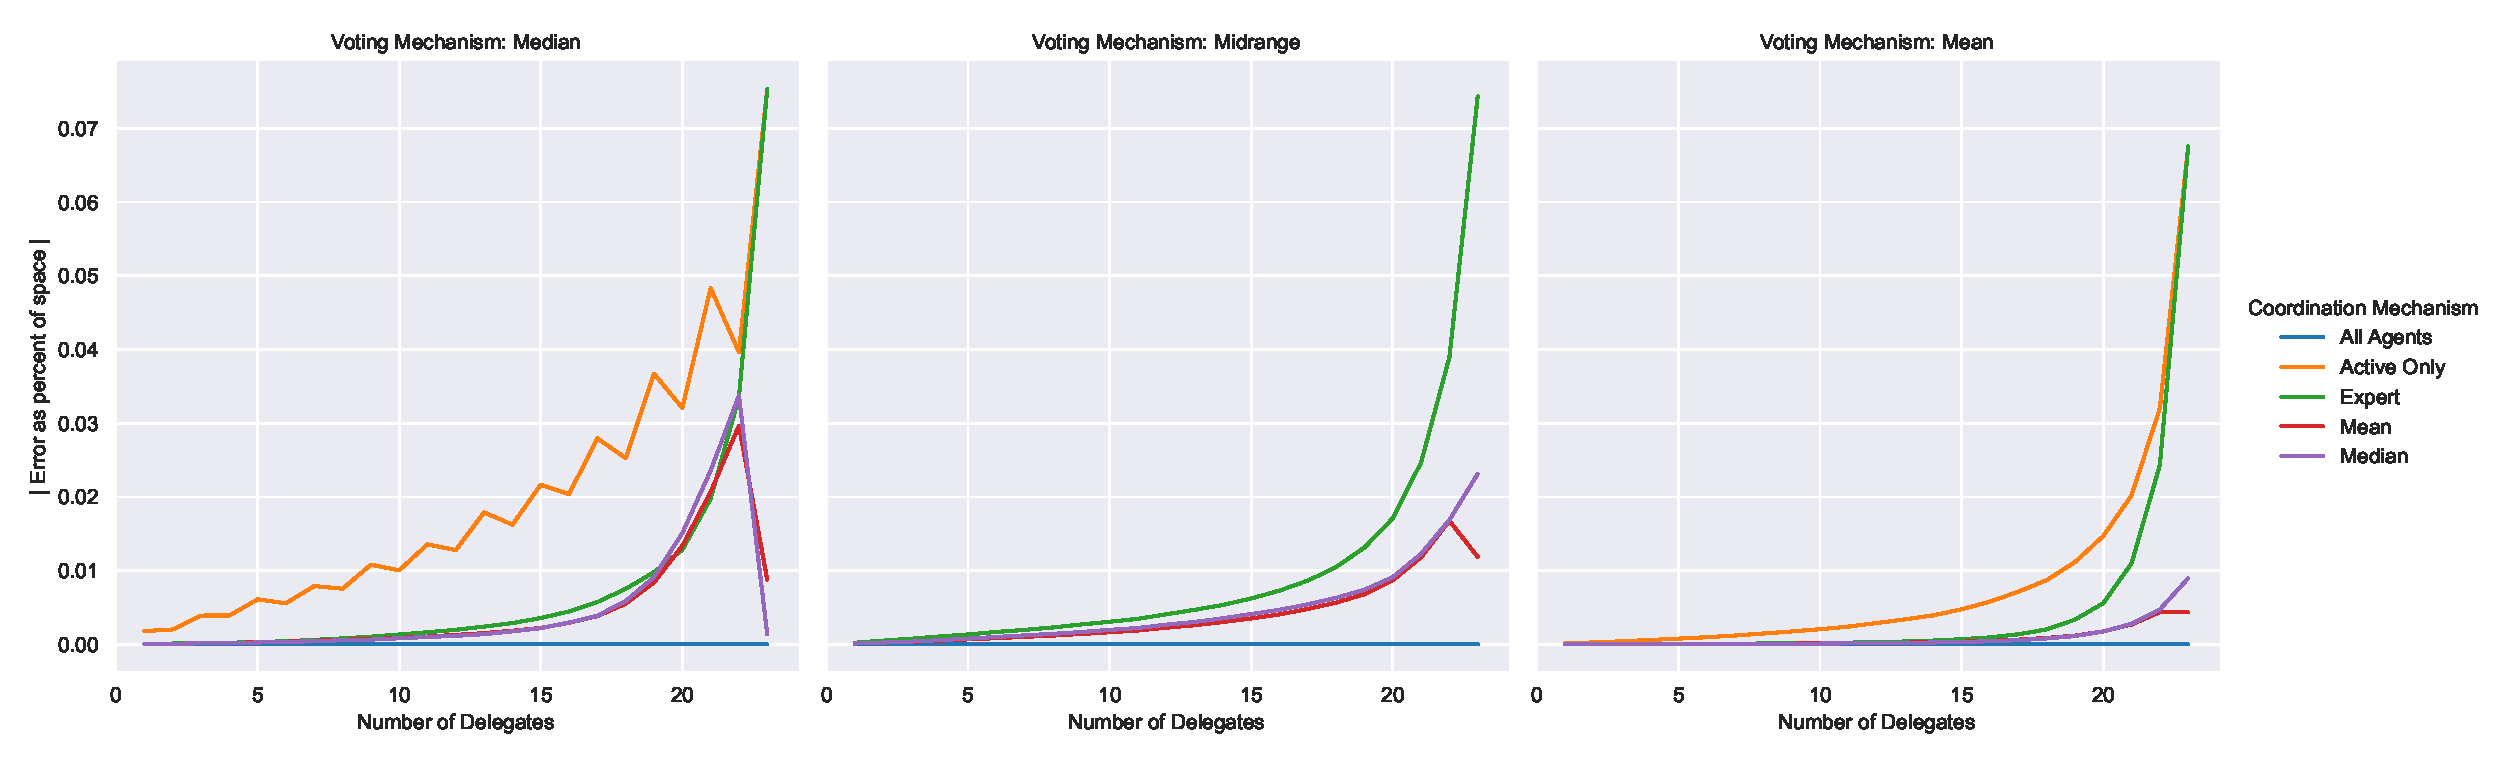
\includegraphics[scale=0.55]
        {content/chapter2/figures/vm_col_cm_hue_error_as_percent_of_space_abs_mean}
        \caption{
            The absolute mean error by coordination mechanism per voting mechanism.
            Note All Agents represents when all agents are voting, meaning no proxy
            voting is used and all agents are present.
            Similarly, Active Only represents when proxy voting is not used and not
            all agents are present, and when proxies lose their constituents.
        }
        \label{fig:vm-col-cm-hue-error-as-percent-of-space-abs-mean}
    \end{figure}
\end{landscape}

% \section{Conclusions}\label{sec:conclusions}?
% \section{Future Work}\label{sec:future-work}?

    \section{Conclusions}\label{sec:conclusions}
We have shown proxy voting is able to produce low-error results, even when the
delegating portion of the population is large.
We have additionally shown the Mean voting mechanism with the Mean and Median
coordination mechanisms achieve the lowest error.
These mechanism combinations are generally able to produce results with less than a 5\%
change in outcome when the delegating portion is more than half the total
population, and produce considerably less when the delegating portion is lower.

We have additionally shown proxy voting is at its weakest with highly polarized
topics, such as those represented by \betadistribution{0.3}{0.3}.
In these cases, agents should make an extra effort to participate in deliberation and
vote in-person instead of by proxy.
While proxy voting is still better than not voting, if agents are unable to vote
in-person, it may be wise to find an alternative to proxy voting on such divisive
topics.

Proxy voting also appears to be effective, even when preferences change.
Error continues to be minimized after agents change their preference compared to only
active agents voting, even when they are unable to change their delegates.

Finally, we have shown that proxy voting is a powerful tool that consistently
performs better than not allowing inactive agents to vote.
By employing proxy voting, systems will be able to maintain their accuracy while
increasing the total system utility.

% \section{Future Work}\label{sec:future-work}?


    % Endmatter
% For BibTeX references: specify a .bib file and a style.
% The style used here is for IEEE transactions formatting:
\references{references/IEEEabrv,references/research}{IEEEtran}

    %
%  Example Appendix pages.
%  Modified to use new usu-thesis-mk2 appendix facilities.
%
%  Time-stamp: "[appendix.tex] last modified by Scott Budge (scott) on
%  2021-06-28 (Monday, 28 June 2021) at 09:03:44 on goga.ece.usu.edu"
%
%  Info: $Id: appendix.tex 1183 2021-06-28 16:49:30Z scott $   USU
%  Revision: $Rev: 1183 $
% $LastChangedDate: 2021-06-28 10:49:30 -0600 (Mon, 28 Jun 2021) $
% $LastChangedBy: scott $
%
%
% For a single appendix, use \makeappendix, and place the 
% body of the appendix after it

%\makeappendix

% < single appendix body here >

% For multiple appendices, use \makeappendices, and create each appendix
% using \appendix{}
% For sub-appendices use \appendixsection{} and \appendixsubsection{}

\makeappendices
\appendix{Voting Distributions}\label{chap:voting-distributions}

\appendixsection{Percent inside Extents}
% TODO: Add description of table
This is placeholder text to ensure
\autoref{tab:distributions-percent-inside-extents} stays in the correct
location. % FIXME

% - Distribution of votes
%     - Uniform
%     - Gaussian
%     - Bimodal about center
%     - Skewed?

\begin{table}[htbp]
    % increase table row spacing, adjust to taste
    \renewcommand{\arraystretch}{1.3}

    \caption{List of distributions used by agents to vote.}
    \label{tab:distributions-percent-inside-extents}

    \centering
    \begin{tabular}{|c|c|c|}
        \hline
        Distribution      & Notation      & Percent inside Extents \\
        \hline
        Uniform           & \uniformdist  & 100\%                  \\
        \hline
        Normal (Gaussian) & \gaussiandist & 99.7\%                 \\
        \hline
        Beta              & \betadist     & 100\%                  \\
        \hline
    \end{tabular}
\end{table}

\appendixsection{Distributions used}
% TODO: Add graphs of distributions used
\begin{table}[htbp]
    % increase table row spacing, adjust to taste
    \renewcommand{\arraystretch}{1.3}

    \caption{List of distributions used by agents to vote.}
    \label{tab:distributions}

    \centering
    \begin{tabular}{|c|c|c|}
    \end{tabular}
\end{table}

\appendixsection{Distributions of Error}
The distribution of square error for each voting mechanism is displayed as a
KDE graph in \autoref{fig:voting_mechanisms_distribution}.

\begin{figure}[!t]
    \centering
    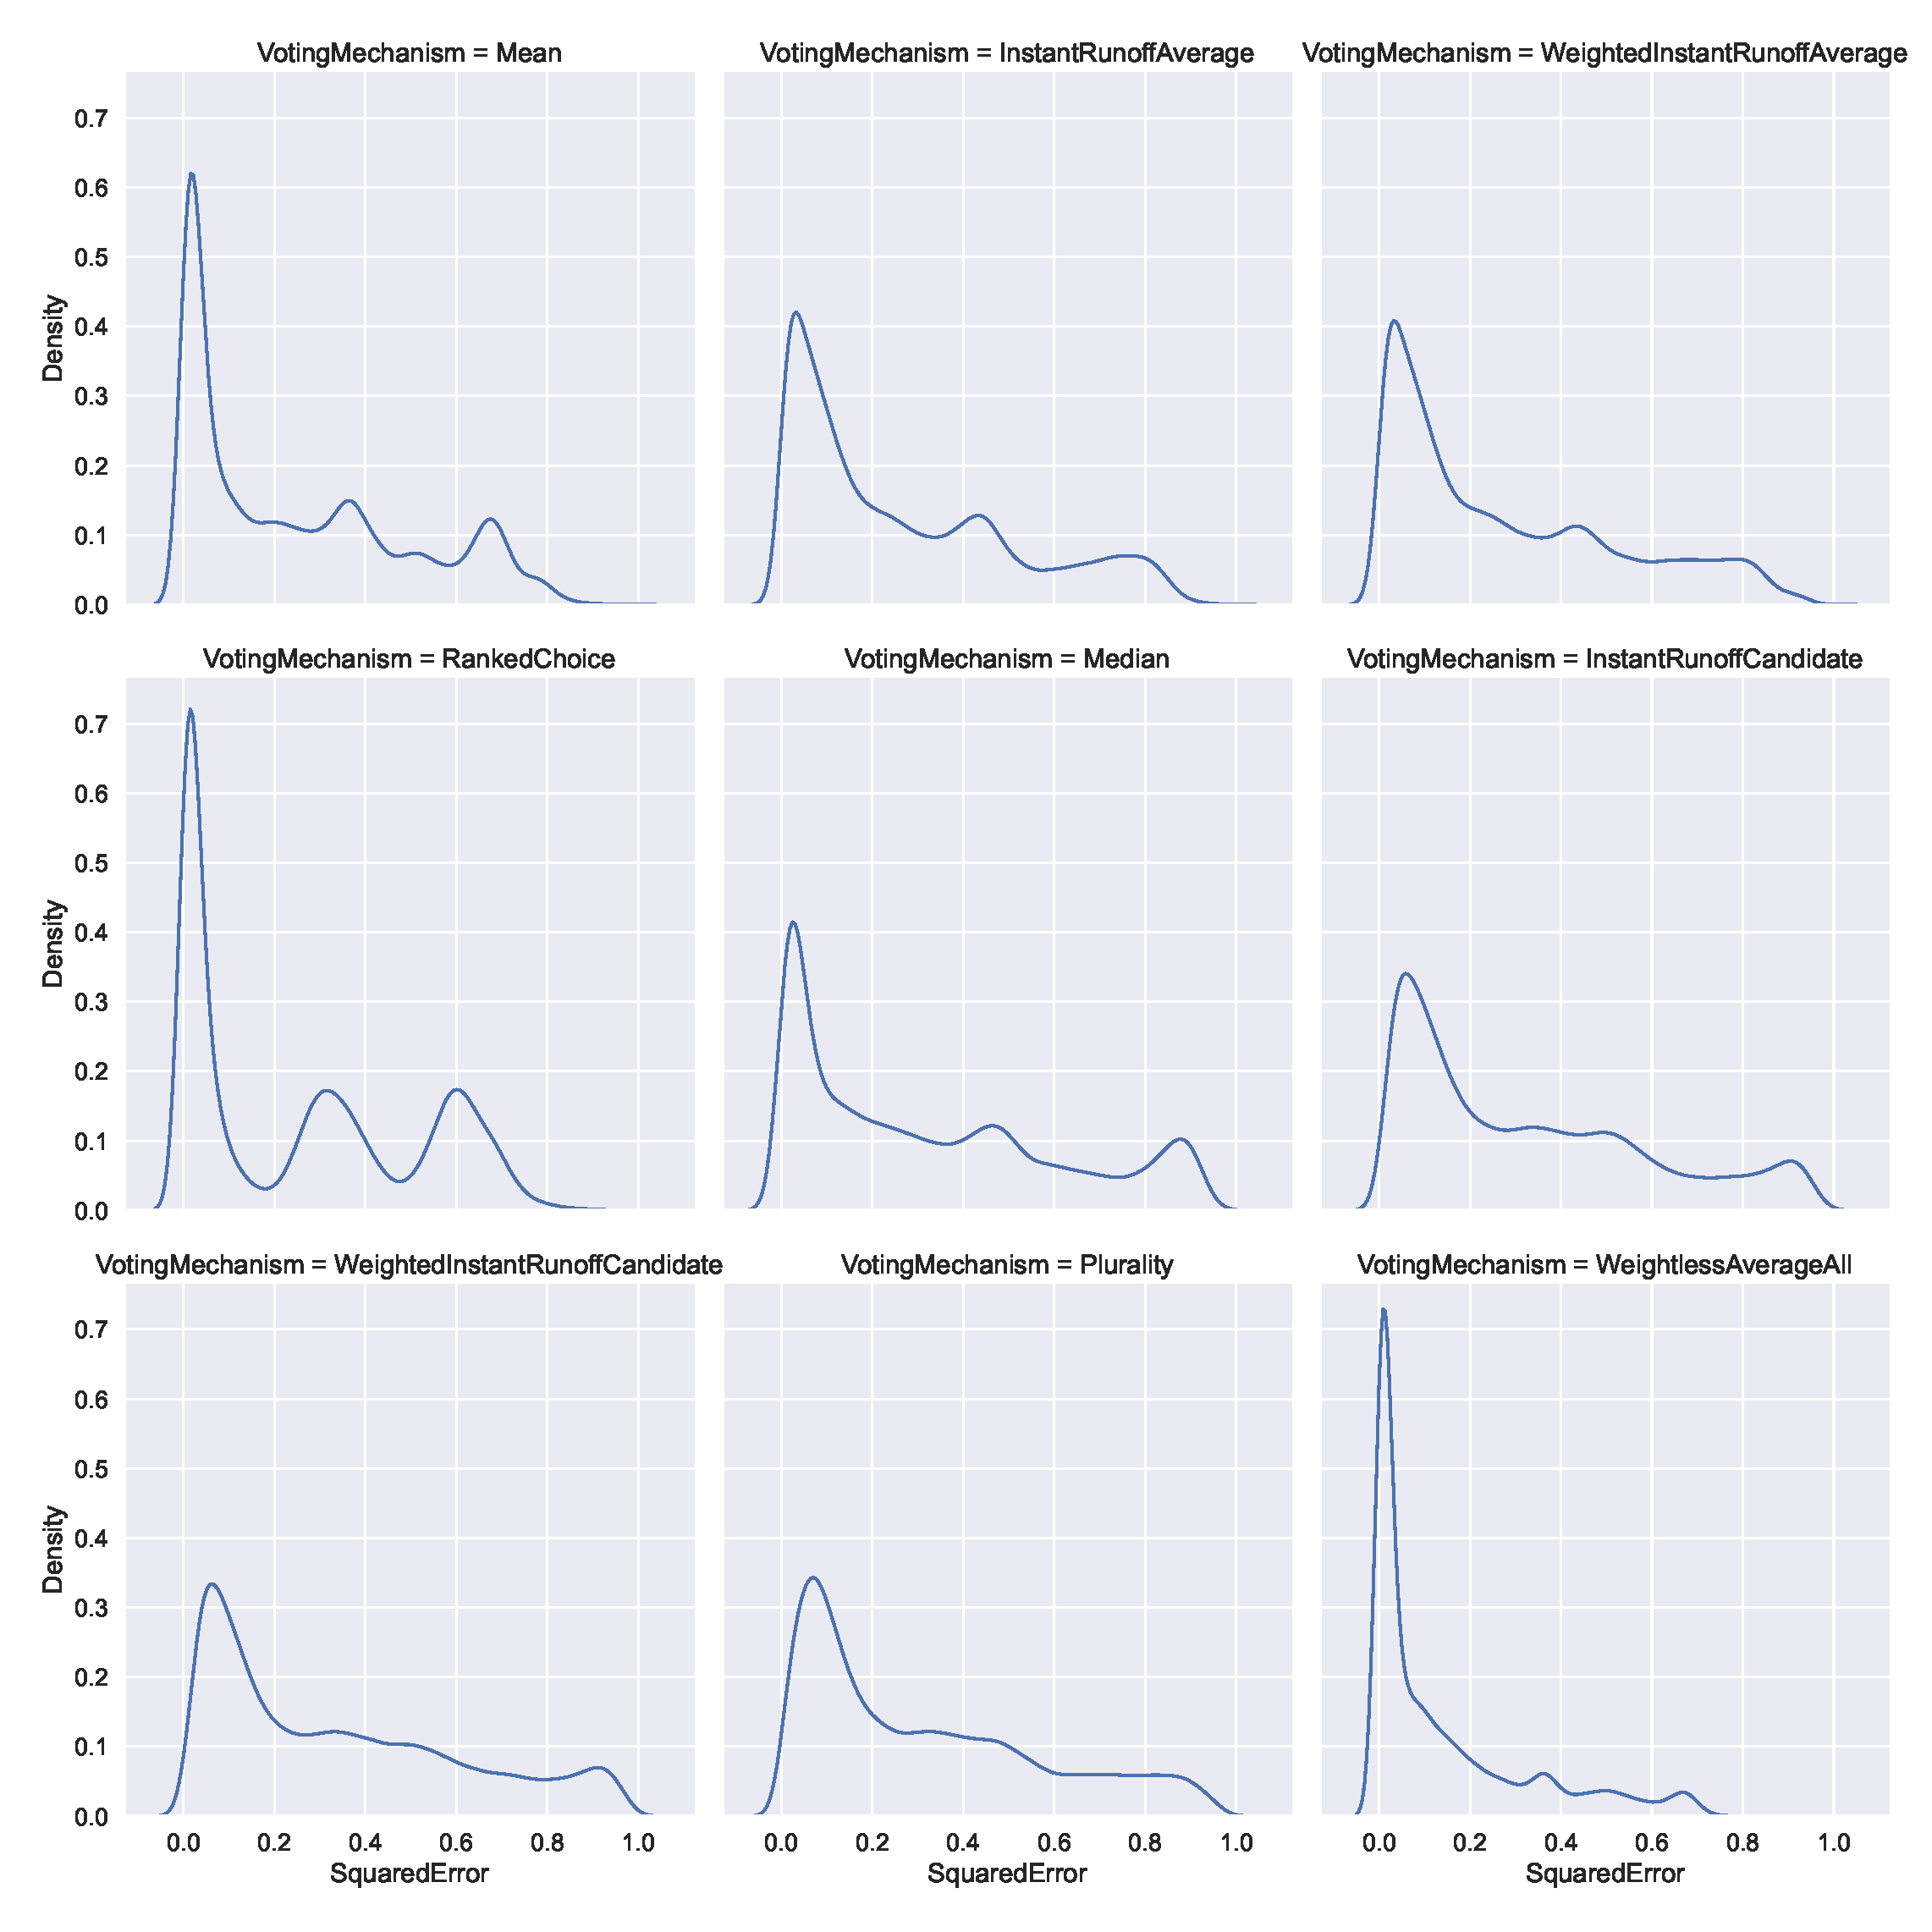
\includegraphics[
        width=\textwidth,
        height=\dimexpr
        \textheight - 2 % Could also be .9\textheight
        \baselineskip,
        keepaspectratio]
    {./content/figures/voting_mechanisms_distribution}
    \caption{The distribution of squared error by voting mechanism}
    \label{fig:voting_mechanisms_distribution}
\end{figure}

\end{document}
